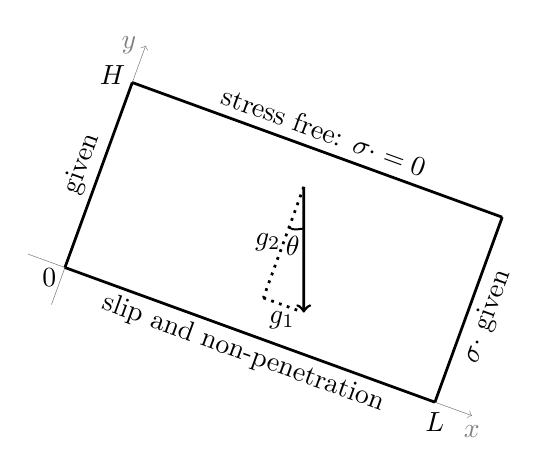
\begin{tikzpicture}[scale=2.5,rotate=-20]
  % axes
  \draw[->,gray,very thin] (-0.2,0.0) -- (2.2,0.0) node[below] {$x$};
  \draw[->,gray,very thin] (0.0,-0.2) -- (0.0,1.2) node[left] {$y$};

  % labeled rectangle
  \draw[line width=1.0pt] (0.0,0.0) -- (2.0,0.0);
  \draw[line width=1.0pt] (0.0,1.0) -- (2.0,1.0);
  \node[xshift=-0.2cm,yshift=-0.13cm] at (0.0,0.0) {$0$};
  \node[xshift=0.0cm,yshift=-0.25cm] at (2.0,0.0) {$L$};
  \node[xshift=-0.25cm,yshift=0.1cm] at (0.0,1.0) {$H$};
  \draw[line width=1.0pt] (0.0,0.0) -- (0.0,1.0);
  \draw[line width=1.0pt] (2.0,0.0) -- (2.0,1.0);

  % boundary conditions
  \node[rotate=70] at (-0.1,0.5) {$\bu$ given};
  \node[rotate=70] at (2.1,0.5) {$\sigma\cdot\bn$ given};
  \node[rotate=-20] at (1.0,1.1) {stress free: $\sigma\cdot\bn=0$};
  \node[rotate=-20] at (1.0,-0.1) {slip and non-penetration};
  % slip is $\bt \cdot \sigma \cdot \bn$ given
  % non-penetration is $\bu\cdot\bn=0$

  % gravity diagram
  \draw[line width=1.0pt,dotted] (1.0,0.8) -- node[xshift=-0.2cm,yshift=0.0cm] {$g_2$} (1.0,0.2);
  \draw[line width=1.0pt,dotted] (1.0,0.2) -- node[xshift=0.0cm,yshift=-0.2cm] {$g_1$} (1.2,0.2);
  %>> 0.6 * tan((pi/180)*20)
  %ans =  0.21838
  \draw[->,line width=1.0pt] (1.0,0.8) -- (1.21838,0.2) node[xshift=0.2cm,yshift=0.6cm] {$\bg$};
  \draw[line width=0.7pt] (1.0,0.58) .. controls (1.03,0.575) and (1.04,0.585) .. (1.07,0.6);
  \node at (1.05,0.5) {$\theta$};
\end{tikzpicture}

